\documentclass[tikz,border=5]{standalone}
\usepackage{amsmath, amsthm, amssymb,enumerate}
\usepackage{tikz}
\usetikzlibrary{shapes,arrows,fit,calc,positioning,patterns}
\usepackage{xcolor}
\usepackage{tikz}
\usepackage{pgfplots,amsmath}
\usetikzlibrary{shapes,arrows,fit,calc,positioning,patterns,decorations.pathmorphing,decorations.pathreplacing}
\tikzset{ brokenrect/.style={

    append after command={

      \pgfextra{

      \path[draw,#1]

       decorate[decoration={zigzag,segment length=0.3em, amplitude=.7mm}]

       {(\tikzlastnode.north east)--(\tikzlastnode.south east)}      

        -- (\tikzlastnode.south west)|-cycle;

        }}}}
\tikzset{ brokenrect2/.style={

    append after command={

      \pgfextra{

      \path[draw,#1]

       decorate[decoration={zigzag,segment length=0.3em, amplitude=.7mm}]

       {(\tikzlastnode.north west)--(\tikzlastnode.south west)}      

        -- (\tikzlastnode.south east)|-cycle;

        }}}}
\tikzset{cross/.style={cross out, draw=black, minimum size=2*(#1-\pgflinewidth), inner sep=0pt, outer sep=0pt},
%default radius will be 1pt. 
cross/.default={1pt}}

\begin{document}

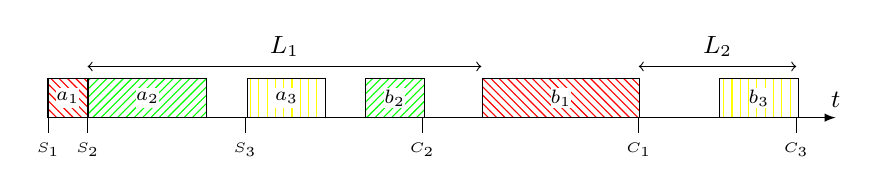
\begin{tikzpicture}

\def\ox{0} 
\def\oy{0} 
\coordinate(o) at (\ox,\oy);

%axis
\def\tl{10.0}
\draw [-latex](\ox,\oy) node[above left]{} -- (\ox+\tl,\oy) node[above,font=\small]{$t$};



%definitions for jobs
\def\pi{0.5}
\tikzstyle{mystyle}=[draw, minimum height=0.5cm,rectangle, inner sep=0pt,font=\scriptsize]
\tikzstyle{mystyle2}=[draw = none, minimum height=0.25cm,rectangle, inner sep=0pt,font=\scriptsize]


\draw (0,0) -- (0,-0.2) node[below] {\tiny $S_1$};
\draw (\pi,0) -- (\pi,-0.2) node[below] {\tiny $S_2$};
\draw (2.5,0) -- (2.5,-0.2) node[below] {\tiny $S_3$};
\draw (7.5,0) -- (7.5,-0.2) node[below] {\tiny $C_1$};
\draw (4.75,0) -- (4.75,-0.2) node[below] {\tiny $C_2$};
\draw (9.5,0) -- (9.5,-0.2) node[below] {\tiny $C_3$};

\draw [<->] (\pi,0.65)--node[above]{\small $L_1$}(\pi+5,0.65);
\draw [<->] (7.5,0.65)--node[above]{\small $L_2$}(9.5,0.65);

%jobs
\node(b1) [above right=-0.01cm and -0.01cm of o,mystyle, minimum width=\pi cm,pattern=north west lines, pattern color=red]{};
\node(b1_t) [mystyle2, fill = white] at (b1.center) {$a_1$};
\node(b2) [right=5cm of b1,mystyle, minimum width=2 cm,pattern=north west lines, pattern color=red]{};
\node(b2_t) [mystyle2, fill = white] at (b2.center) {$b_1$};
\node(b3) [right=0cm of b1,mystyle, minimum width=1.5 cm,pattern=north east lines, pattern color=green]{};
\node(b3_t) [mystyle2, fill = white] at (b3.center) {$a_2$};
\node(b4) [right=2cm of b3,mystyle, minimum width=0.75 cm,pattern=north east lines, pattern color=green]{};
\node(b4_t) [mystyle2, fill = white] at (b4.center) {$b_2$};
\node(b5) [right=0.5cm of b3,mystyle, minimum width=1 cm,pattern=vertical lines, pattern color=yellow]{};
\node(b5_t) [mystyle2, fill = white] at (b5.center) {$a_3$};
\node(b6) [right=1cm of b2,mystyle, minimum width=1 cm,pattern=vertical lines, pattern color=yellow]{};
\node(b6_t) [mystyle2, fill = white] at (b6.center) {$b_3$};
\end{tikzpicture}

\end{document}